\chapter{Sprint0: Analyse et spécification des besoins}

%%% %%%%%%%%% %%%
\section*{Introduction}
Après аvoir présenté le cadre général et la méthodologie agile utilisée durant notre projet, nous présentons le sprint 0 qui a duré 2 semaines. Dans cette partie de ce chapitre, nous présentons les besoins fonctionnels et non fonctionnels du projet.
%%%%%%%%%%
\section{Analyse et spécification des besoins}
Dans cette partie, nous commençons par présenter tous les besoins que notre projet tourne autour desquels et qu’il doit les satisfaire. Ensuite, nous allons introduire les exigences fonctionnelles et non-fonctionnelles, et le diagramme de cas d’utilisation générаle.
\subsection{Besoins fonctionnels}
Le système réalisé dans le cadre de ce projet doit offrir à l’administrateur les possibilités suivantes :
\newpage
                \begin{itemize}
                \item Accélérer la distribution de l’offre en fluidifiant les parcours, de la mise en marché à la vente multicanal.
                \item Simplifier les processus de gestion et l’expérience de l’assuré.
                \item Enrichir cette expérience en proposant de nouveaux services digitaux répondant aux nouveaux usages.
                \end{itemize}



\subsection{Diagrammes de cas d’utilisation général}
Après avoir dégagé les différents acteurs en interaction avec notre système et les exigences fonctionnels et non fonctionnels, nous allons présenter ces différentes fonctionnalités avec le diagramme de cas d’utilisation général 
\begin{figure}[H]
\centering
\frame{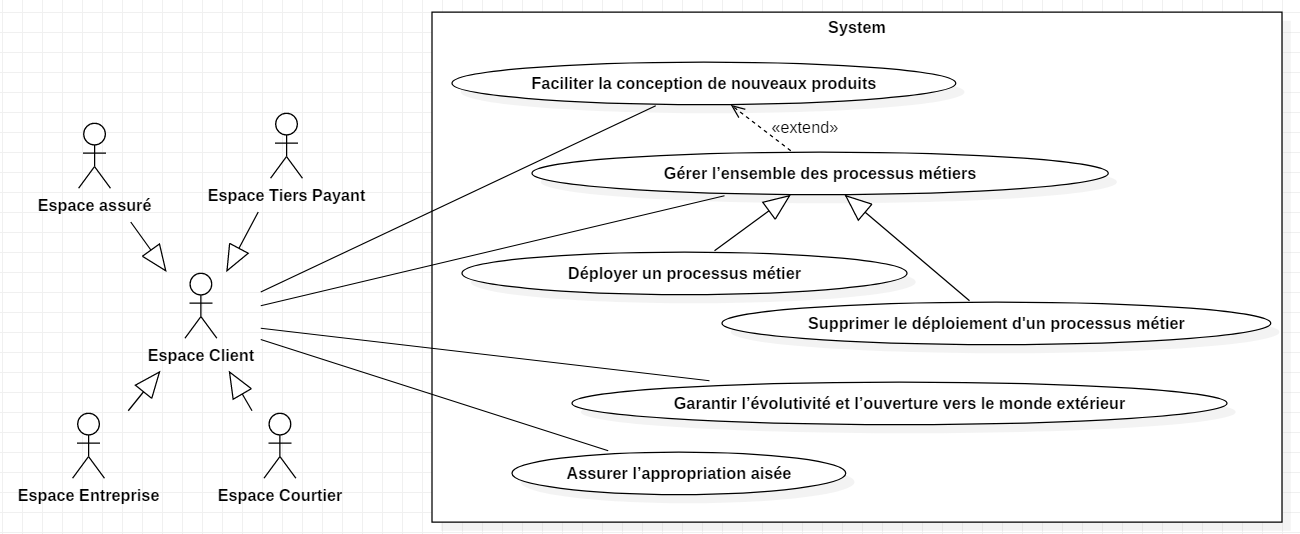
\includegraphics[width=1.1\columnwidth,height=0.7
\columnwidth]{images/use.png}}
\caption{Diagramme de cas d’utilisation général}
\end{figure}

\subsection{Besoins non-fonctionnels}
Les besoins non fonctionnels décrivent toutes les contraintes techniques, ergonomiques et esthétiques auxquelles est soumis le système pour sa réalisation et pour son bon fonctionnement. Et ce qui concerne notre application, nous avons dégagé le besoins suivants :

\begin{itemize}[font=\normalsize]
                \ding{226}\textbf{Fiabilité et pertinence :} les services doivent fournir des résultats corrects et pertinents.
                \end{itemize}
\begin{itemize}[font=\normalsize]
                \ding{226}\textbf{Temps réel :} la solution doit fournir les ressources demandées en temps réel.
                \end{itemize}
\begin{itemize}[font=\normalsize]
                \ding{226}\textbf{Maintenаbilité :} la maintenabilité et l’évolutivité sont obligаtoires pour avoir un logiciel de qualité.
                \end{itemize}
\begin{itemize}[font=\normalsize]
                \ding{226}\textbf{Lisibilité d’un code source :} Le code de l’applicаtion doit être lisible et compréhensible afin de garantir la maintenance de l’application en cas de besoin.
                \end{itemize}
\begin{itemize}[font=\normalsize]
                \ding{226}\textbf{Performance :} le système doit être stable et son temps de réponse doit être tolérable.
                \end{itemize}
\begin{itemize}[font=\normalsize]
                \ding{226}\textbf{Ergonomie :} L’interface utilisateur doit être claire et facile à manipuler
                \end{itemize}

\section{L’architecture logique}
\subsection{D Health}
\subsubsection{\Large Pour Qui ?}
D HEALTH est dédié aux assureurs traditionnels, aux mutuelles, aux
courtiers, distributeurs, banques, sociétés de gestion et institutions
de prévoyance.
D HEALTH couvre toute la chaîne de valeur (Clients, Partenaires,
Distributeurs, Gestionnaires, Tiers) , en plus des fonctionnalités
basiques D HEALTH permet également de :
\begin{itemize}[font=\normalsize]
                \ding{226}\textbf{Faciliter la conception de nouveaux produits }
                
\end{itemize}
\begin{itemize}[font=\normalsize]
                \ding{226}\textbf{Permettre la configuration de l’ensemble des processus métiers}
                \end{itemize}
                \begin{itemize}[font=\normalsize]
                \ding{226}\textbf{Garantir l’évolutivité et l’ouverture vers le monde extérieur}
                \end{itemize}
                \begin{itemize}[font=\normalsize]
                \ding{226}\textbf{Assurer l’appropriation aisée par les utilisateurs du système
d’information}
                \end{itemize}
                \subsubsection{Nos Atouts ?}
                \begin{itemize}[font=\normalsize]
                 \ding{226}\textbf{la performance :} robustesse, traçabilité ...
                 \end{itemize}
                 \begin{itemize}[font=\normalsize]
                  \ding{226}\textbf{la sécurité et conformité réglementaire}
                  \end{itemize}
                  \begin{itemize}[font=\normalsize]
                   \ding{226}\textbf{la flexibilité du modèle :} SaaS, PaaS ou IaaS
                   \end{itemize}
                   \begin{itemize}[font=\normalsize]
                    \ding{226}\textbf{l’innovation :} Ateliers produits,
User expérience,
OCR,
workflows paramétrables,
détection de la fraude,
Contrôle de la qualité des données.
                    \end{itemize}
                    \begin{itemize}[font=\normalsize]
                     \ding{226}\textbf{User Expérience}
                     \end{itemize}
                     
                \begin{figure}[H]
\centering
\frame{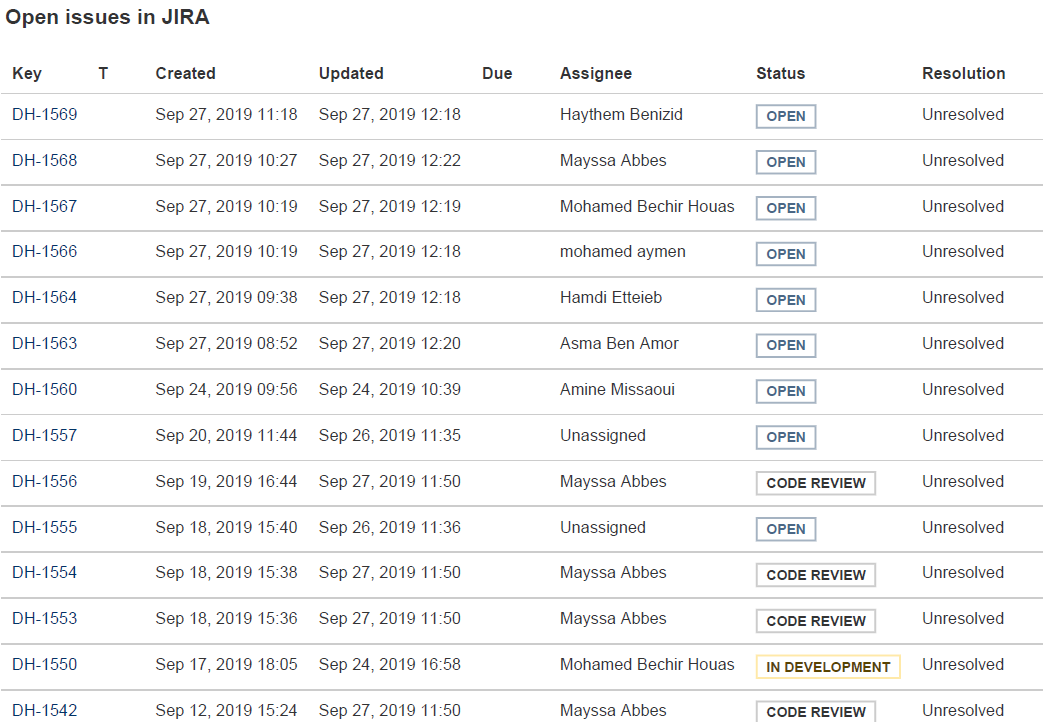
\includegraphics[width=1\columnwidth,height=0.6
\columnwidth]{images/les9.png}}
\caption{Open issues in JIRA}
\label{fig:Mod-Enseig}
\end{figure}
                      
\subsection{D Suite}     
Dans un contexte économique de plus en plus concurrentiel, les acteurs de l’assurance sont confrontés à une clientèle exigeante,
renseignée et plus volatile. Depuis la mise en vigueur de la loi Hamon et le développement des comparateurs d’assurance, les assurés ont la
possibilité de changer de prestataire d’assurance en un claquement de doigts.
Pour anticiper et se prémunir de la fuite de leurs clients, les assureurs mettent en place des solutions de gestion de la relation client permettant
de répondre à une politique de satisfaction plus stricte. Afin de rendre cet objectif atteignable, les acteurs de l’assurance développent une
stratégie d’accompagnement des assurés depuis la souscription d’un contrat jusqu’à sa résiliation.
D Suite d'outils et d'application web proposée par Dqlick qui est  compatible avec D Health et qui touchent plusieurs domaines :

\begin{itemize}[font=\normalsize]
                 \ding{226}\textbf{Espace assuré}
                 \end{itemize}
                 \begin{itemize}[font=\normalsize]
                  \ding{226}\textbf{Espace Entreprise}
                  \end{itemize}
                  \begin{itemize}[font=\normalsize]
                   \ding{226}\textbf{Espace Courtier}
                   \end{itemize}
                   \begin{itemize}[font=\normalsize]
                    \ding{226}\textbf{Espace Tiers Payant}
                 \end{itemize}
                 \begin{itemize}[font=\normalsize]
                  \ding{226}\textbf{Outil aide à la vente}
                  \end{itemize}
                  \begin{itemize}[font=\normalsize]
                   \ding{226}\textbf{E-Devis}
                   \end{itemize}
                   \begin{itemize}[font=\normalsize]
                  \ding{226}\textbf{GED}
                  \end{itemize}
                  \begin{itemize}[font=\normalsize]
                   \ding{226}\textbf{Espace Administration des assurés}
                   \end{itemize}
                   
                                   \begin{figure}[H]
\centering
\frame{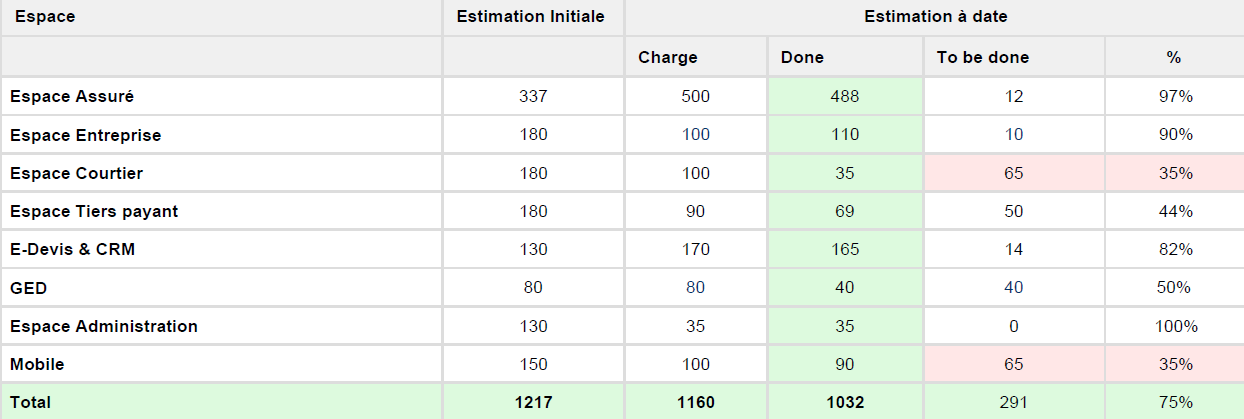
\includegraphics[width=1\columnwidth,height=0.6
\columnwidth]{images/les10.png}}
\caption{Gestion Projet}
\label{fig:Mod-Enseig}
\end{figure}
                                   \begin{figure}[H]
\centering
\frame{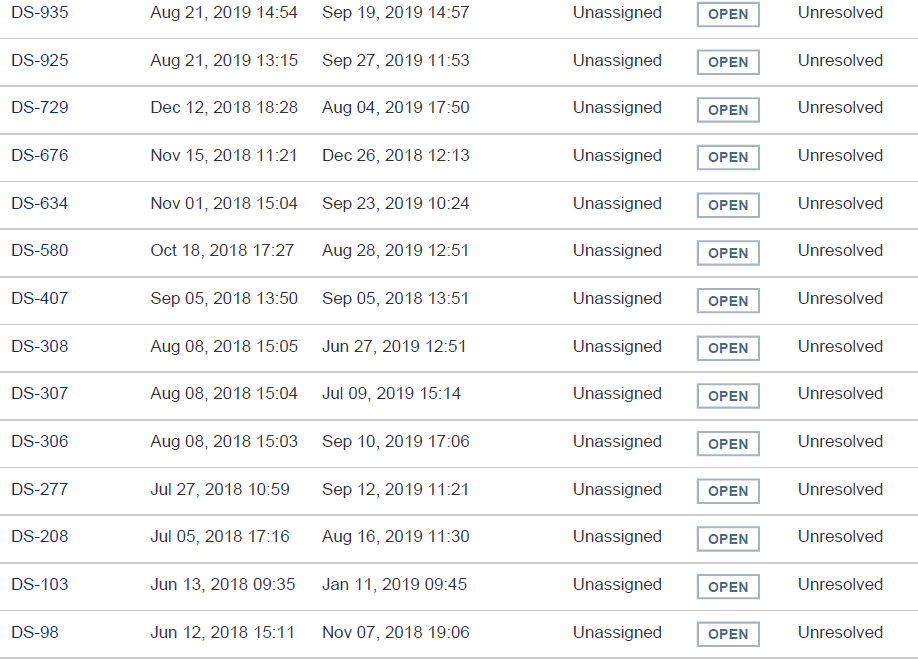
\includegraphics[width=1\columnwidth,height=0.6
\columnwidth]{images/les11.png}}
\caption{Open issues in JIRA}
\label{fig:Mod-Enseig}
\end{figure}
                   



\section*{Conclusion}
Dans ce chapitre nous avons identifié les besoins fonctionnels et non fonctionnels de notre projet. Nous avons construit l’architecture logique
D Health et D Suite de notre solution.